\documentclass[10pt,a4paper]{article}
\usepackage[utf8]{inputenc}
\usepackage[polish]{babel}
\usepackage[T1]{fontenc}
\usepackage{amsmath}
\usepackage{amsfonts}
\usepackage{amssymb}
\usepackage{graphicx}
\usepackage{epsf} 
\usepackage{float}
\usepackage{booktabs}
\usepackage[a4paper]{geometry}
\nonstopmode

\title{Flow-Shop Scheduling\\Laboratorium Optymalizacji Kombinatorycznej}

\begin{document}
\newgeometry{left=3cm, bottom=3cm, top=3cm}
\maketitle
\begin{center}
\Large{Szymon Gramza}\\
szymon.gramza@student.put.poznan.pl\\
\vspace{4mm}
\Large{Maciej Sobkowski}\\
maciej.sobkowski@student.put.poznan.pl\\
\vspace{5mm}
\Large{Prowadzący: Marcin Radom}\\  
\end{center}


\vspace{10mm}
\section{Wprowadzenie}
\subsection{Opis problemu}
Problem Flow-Shop jest problemem optymalizacji kobminatorycznej, który polega na
szeregowaniu zadań przy wykorzystaniu ustalonej liczby maszyn. Każde zadanie
składa się z listy operacji, które muszą zostać wykonane w określonej kolejności
na określonej maszynie, a każdą operację cechuje czas wykonywania. Zadania
pojawiają się w różnych momentach pracy systemu, a maszyny na których są
wykonywane posiadają wymuszone przestoje.  Do rozwiązania powyższego problemu
wykorzystaliśmy zainspirowaną zachowaniem się mrówek poszukujących pożywienia
metaheurystykę ACO\@. Algorytm mrówkowy będziemy porównywać z rozwiązaniem
uzyskanym za pomocą algorytmów losowego oraz rozwiązaniem optymalnym obliczonym
za pomocą wzoru: 
\begin{equation}
  opt = \frac{\text{suma\ czasów\ wszystkich\ operacji}}{\text{liczba\ maszyn}}
\end{equation}

\subsection{Program testujący}

\subsubsection{Opis}
Aplikacja została napisana w języku C i wykorzystuje biblioteki dostępne w
systemach z rodziny GNU/Linux. 

\subsubsection{Kompilacja}
Kompilacja została zautomatyzowana przy pomocy programu GNU Make. Aby
skompilować program należy przejść do katalogu \textit{scheduler} i z poziomu 
konsoli wydać polecenie \textit{make}. Prawidłowe zakończenie procesu kompilacji 
zostanie zasygnalizowane komunikatem \textit{Zakończono linkowanie!}. W ten sam
sposób należy przebiega kompilacja programu \textit{generator}.

\subsubsection{Uruchomienie}
Praca aplikacji jest sterowana przez przełączniki powszechnie stosowane w
oprogramowaniu linuksowym.  Przykładowe wywołanie \textit{scheduler -i
inst\_name -o file\_name.csv} uruchomi program dla instancji zapisanej w pliku
inst\_name i wykona algorytm ACO oraz losowy. Wynik szeregowania zostanie
zapisany do pliku o nazwie file\_name.csv.  Dodatkowo, aby uruchomić program
generujący instancje należy użyć polecenia \textit{./generator}.\\ Przykładowe wywołanie:
\textit{./generator -i input\_name -o inst\_name } spowoduje wygenerowanie pliku
instancji inst\_name przyjmując parametry zawarte w pliku input\_name zgodnie ze
schematem, że każda linia składa się z 5 liczb całkowitych, które odpowiednio
charakteryzują: liczbę zadań, początek i koniec przedziału czasu wykonania
operacji, początek i koniec przedziału czasu gotowości zadania.\\ Generator
losuje czasy wykonania operacji i czasy gotowości dla zdefiniowanej liczby
zadań.

\section{Algorytm Ant Colony Optimization}

\subsection{Opis algorytmu}
Zastosowana przez nas metaheurystyka - Ant Colony Optimization - opiera się na
naturalnym zachowaniu kolonii mrówek poszukujących pożywienia. Algorytm korzysta
ze struktur utrzymujących informację o drodze od źródła do celu, przebytej przez
każdą mrówkę danego pokolenia. Algorytm został zaprojektowany do problemów
znajdowania ścieżki w grafie o najmniejszym koszcie (problem TSP).
Przystosowanie algorytmu do problemu szeregowania zadań sprowadza się w naszym
przypadku do przedstawienia operacji danej instancji w postaci grafu, którego
przykład umieszczono poniżej:\\
\begin{center}
    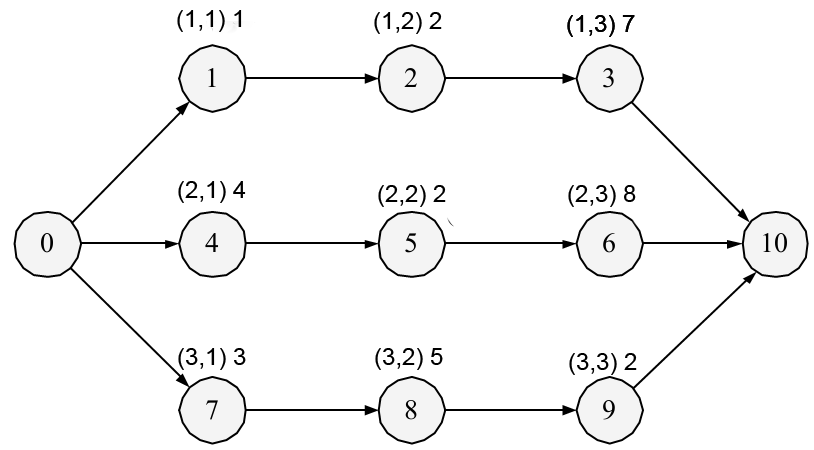
\includegraphics[scale=0.4]{./figures/pic01.png}\\
\end{center}
Każdemu wierzchołkowi grafu przyporządkowana jest jedna operacja, każda
operacja zaś posiada informacje o maszynie i numerze zadania.  Zależności
pomiędzy kolejnością wykonania operacji reprezentują łuki między nimi, ponadto
graf posiado dwa dodatkowe wierzchołki - początkowy i końcowy - które pozwalają
przypisać pierwszej i ostatniej operacji feromon. Dzięki takiej reprezentacji
problemu możemy korzystać z wzorów przeznaczonych dla algorytmu TSP z drobnymi
modyfikacjami.

Informacje o ilości feromonów utrzymywane są w macierzy NxN (N - liczba
operacji).  Rozwiązaniem generowanym przez mrówkę jest łańcuch wszystkich
wierzchołków zachowujący zależnosci między operacjami w zadaniu.  (sortowanie
topologiczne) Przykładowy łańcuch: [0 1 4 2 7 5 8 3 6 9 10].

Przed uruchomieniam właściwego algorytmu, początkowa ilość feromonu na każdej
ścieżce przyjmuje bardzo małą wartość, w naszej implementacji przyjęliśmy $
\tau_0 = 0.001 $ 

\subsubsection{State Transition Rule}
Każda mrówka wybierając drogę stosuję regułę zmiany stanu (State Transition
Rule), którą obrazuje poniższy wzór:\\

\begin{equation}
 s = \left\{ 
  \begin{array}{l l}
    arg\ max_{u \in J(r)} \{ [\tau (r,u)] \cdot [\eta (r,u)^\beta] \} , & \quad
    \text{jeśli $q\leq q_0$}\\
    S, & \quad \text{w przeciwnym razie}
  \end{array} \right.
\end{equation} \\
gdzie:
\begin{itemize}
  \item $ (r,u) $ - łuk od wierzchołka r do u
  \item $ J(r) $ - zbiór wierzchołków dostępnych w punkcie decyzyjnym r
  \item $ \tau (r,u) $ - ilość feromonu na łuku (r,u)
  \item $ \eta (r,u) $ - atrakcyjność łuku (r,u), która w przypadku naszego
    problemu zdefiniowana jest jako odwrotność długości operacji u
  \item $ \beta $ - parametr kontrolujący wpływ atrakcyjności
  \item $ q $ - losowa liczba z przedziału $ \langle 0;1 \rangle $ 
  \item $ q_0 $ - zdefiniowany parametr przyjmujący wartości z przedziału $
    \langle 0;1 \rangle $
  \item $ S $ - zmienna losowa wybierana zgodnia z rozkładem prawdopodobieństwa
    opisanym wzorem (2). 
\end{itemize}
\\
\begin{equation}
 P(r,s) = \left\{ 
  \begin{array}{l l}
    \frac{[\tau (r,s)] \cdot [\eta (r,s)^\beta]}{\sum_{u \in J(r)} {[\tau (r,u)]
    \cdot [\eta (r,u)^\beta]}},
    & \quad \text{jeśli }s \in J(r)\\
     0, & \quad \text{w przeciwnym razie}
  \end{array} \right.
\end{equation}

Powyższa metoda wyboru nosi nazwę pseudoruletki, której zasada działania opiera
się na przydzieleniu wartości procentowej koła ruletki, odpowiadającej
iloczynowi ilości feromonu i atrakcyjności. Po zakręceniu kołem, które jest
równoważne wylosowaniu liczby, wybierany jest następny wierzchołek na drodze
mrówki.

\vspace{15mm}
\subsubsection{Aktualizacja wartości feromonów}
W algorytmie stosujemy dwie strategie aktualizacji feromonów: \\
\begin{enumerate}
  \item lokalna (local updating rule) - w czasie konstruowania ścieżki mrówka
    modyfikuje ilosć feromonu stosując się do poniższego wzoru:\\
  \begin{equation} \tau (r,s) \leftarrow (1 - \rho) \cdot \tau (r,s) + \rho \cdot \tau_0  \end{equation} \\
  gdzie:
  \begin{itemize}
  \item $ \rho $ - współczynnik parowania feromonu (z przedziału $ (0;1) $)
\end{itemize}

  \item globalna (global updating rule) - gdy wszystkie mrówki danej populacji
    dotrą do celu (osiągną końcowy wierzchołek grafu) wartość feromonu jest
    aktualizowana zgodnie ze wzorem:\\
   \begin{equation} \tau (r,s) \leftarrow (1 - \alpha) \cdot \tau (r,s) + \alpha \cdot \Delta \tau (r,s)  \end{equation} \\
  gdzie:
  \begin{itemize}
  \item $ \alpha $ - parametr zaniku feromonu
  \item $ \Delta \tau (r,s) $ - przedstawia się wzorem: \\
  \begin{equation}
 \Delta \tau (r,s) = \left\{ 
  \begin{array}{l l}
    (L_{gb})^{-1} , & \quad \text{jeśli $(r,s) \in$ najlepsza ścieżka}\\
    0, & \quad \text{w przeciwnym razie}
  \end{array} \right.
\end{equation}
  gdzie:
  \item $ L_{gb}$ - długość najlepszej ścieżki ($C_{max}$)
\end{itemize}
\end{enumerate}

\vspace{15mm}
\subsection{Instancje testowe}
Każda znajdująca się poniżej instancja sterowana jest następującymi
parametrami: $ \rho, \alpha, q_0, \tau_0, \beta $.  Klasy instancji
podzieliliśmy na 4 grupy w zależności od rodzaju danych wejściowych: losowe,
rosnące, malejące, v-kształtne.


\newgeometry{left=3cm,top=15mm, bottom=2cm}
%r\restoregeometry
\subsubsection{Różne klasy instancji danych wejściowych.}
\vspace{6 mm}
\begin{center}
\begin{tabular}{|r|l|}
  \hline
  liczba zadań & 50 \\
  czasy operacji & $ \langle 5;100 \rangle $  \\
  liczba mrówek & 10 \\
  liczba pokoleń & 5000 \\
  $ \rho $ & 0.01 \\
  $ \alpha $ & 0.1 \\
  $ q_0 $ & 0.8 \\
  $ \tau_0 $ & 0.001 \\
  $ \beta $ & 2 \\
  \hline
\end{tabular}
\end{center}

\begin{center}
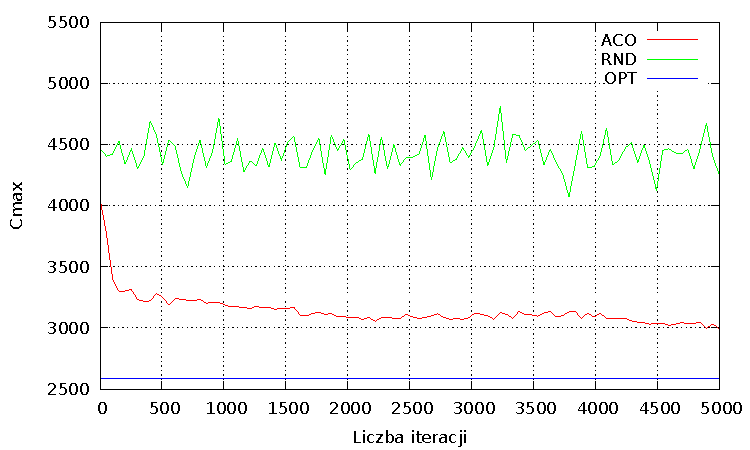
\includegraphics{./figures/inst01_rnd_smooth.pdf}
\vspace{2 mm}
\\losowy}
\\
\vspace{5mm}
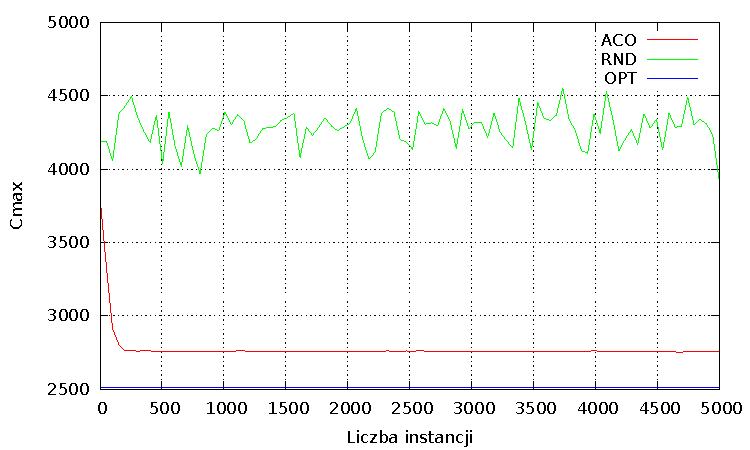
\includegraphics{./figures/inst02_asc_smooth.pdf}
\vspace{2 mm}
\\rosnący

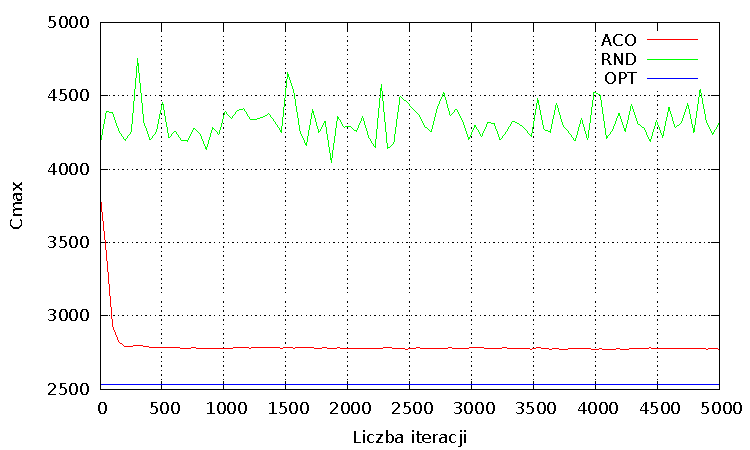
\includegraphics{./figures/inst03_dsc_smooth.pdf}
\vspace{2 mm}
\\malejące
\\
\vspace{5mm}
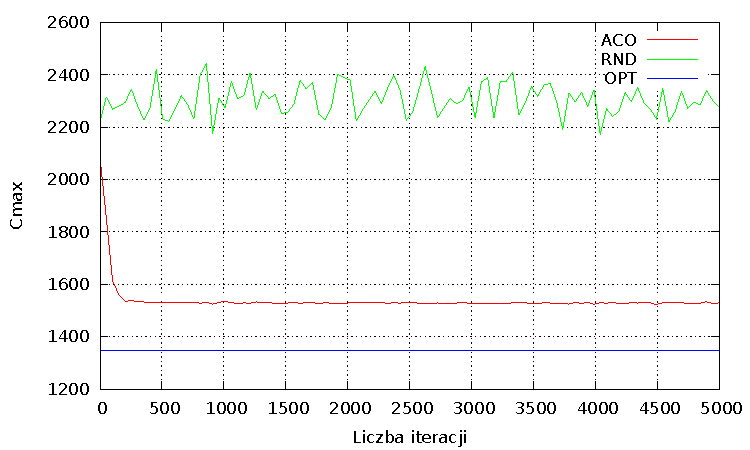
\includegraphics{./figures/inst04_vsh_smooth.pdf}
\vspace{2 mm}
\\v-kształtne

\end{center}
\vspace{8 mm}
Algorytm losowy, niezależnie od rodzaju danych wejściowych oraz ilości iteracji, osiąga średnio podobne wyniki (względna odległość od optimum). Jest to spowodowane brakiem parametrów optymalizujących algorytm losowy. 
Natomiast ACO w kolejnych iteracjach zwraca wynik dążący do optimum. Z analizowanych klas instancji wyróżniają się dane losowe dla których po 5000 iteracji algorytm nie osiąga wyraźnej stabilizacji. Dla pozostałych zestawów danych po około 200 pokoleniach dochodzimy do stabilizacji algorytmu. Wynika to z uporządkowania pozostałych zestawów danych (rosnące/malejące długości kolejnych operacji).

\newpage
\begin{center}
Liczbowe przedstawienie klas instancji
\begin{tabular}{rrrll}
\toprule
\multicolumn{5}{c}{losowe dane}\\
\midrule
Iteracja & ACO & RND  & opt/ACO(\%) & opt/RND(\%) \\
\midrule
50	& 3,796.33	& 4,294.33	& 68.03	& 60.14 \\
1000	& 3,192.15	& 4,419.17	& 80.91	& 58.44 \\
2000	& 3,089.85	& 4,388.67	& 83.59	& 58.85 \\
3000	& 3,101.63	& 4,331.83	& 83.27	& 59.62 \\
4000	& 3,077.53	& 4,458.83	& 83.92	& 57.92 \\
5000	& 3,016.63	& 4,238.50	& 85.61	& 60.93 \\
\bottomrule
\end{tabular}

\begin{tabular}{rrrll}
%opt 2510.333
\toprule
\multicolumn{5}{c}{rosnące dane}\\
\midrule
Iteracja & ACO & RND  & opt/ACO(\%) & opt/RND(\%) \\
\midrule

50	& 3,397.37	& 4,300.33	& 73.89 &	58.38\\
1000	& 2,756.32	& 4,252.50 &	91.08 &	59.03\\
2000	& 2,757.57	& 4,480.17	& 91.03 & 56.03\\
3000	& 2,757.55	& 4,448.83	& 91.03 &	56.43\\
4000	& 2,757.02	& 4,457.83	& 91.05 &	56.31\\
5000	& 2,755.25	& 4,126.83	& 91.11 &	60.83\\
\bottomrule
\end{tabular}

\begin{tabular}{rrrll}
%opt 2528.667
\toprule
\multicolumn{5}{c}{malejące dane}\\
\midrule
Iteracja & ACO & RND  & opt/ACO(\%) & opt/RND(\%) \\
\midrule
50	& 3,418.53	& 4,367.67	& 73.97 &	57.90\\
1000	& 2,778.82	& 4,341.67	& 91.00 &	58.24\\
2000	& 2,780.03	& 4,394.00	& 90.96 & 57.55\\
3000	& 2,777.32	& 4,295.50	& 91.05 &	58.87\\
4000	& 2,770.00	& 4,411.33	& 91.29 &	57.32\\
5000	& 2,774.88	& 4,333.50	& 91.13 &	58.35\\

\bottomrule
\end{tabular}

\begin{tabular}{rrrll}
%opt 1348.333
\toprule
\multicolumn{5}{c}{v-kształtne dane}\\
\midrule
Iteracja & ACO & RND  & opt/ACO(\%) & opt/RND(\%) \\
\midrule
50	& 1,859.73	& 2,282.00	& 72.50 &	59.09\\
1000	& 1,530.27	& 2,277.67	& 88.11 &	59.20\\
2000	& 1,529.47	& 2,341.00 &	88.16 &	57.60\\
3000	& 1,528.95	& 2,304.33 &	88.19 &	58.51\\
4000	& 1,529.55	& 2,340.17 &	88.15 &	57.62\\
5000	& 1,527.00	& 2,268.83 & 88.30 &	59.43\\

\bottomrule
\end{tabular}
\end{center}

\vspace{15mm}
Powyższe tabelki obrazują stosunek wartości optimum do wartości $C_{max}$ w otoczeniach wybranych puntów $\langle numer\ iteracji - 50 ; numer\ iteracji + 50\rangle$, potwierdzając brak optymalizacji rozwiązania w przypadku algorytmu losowego, niezależnie od rodzaju danych wejścciowych.
Zastosowana metaheurystyka natomiast w przypadku danych malejących, rosnących i v-kształtnych ma bardzo podobne osiągi bliskie 90\% wartości optymalnej.
Dane losowe dają gorsze wyniki, osiągając ok. 85\% wartości optymalnej, co jest spowodowane naturą losowego rozkładu danych.


\newpage
\subsubsection{Różne wartości parametru $\beta$.}
\vspace{6 mm}
\begin{center}
\begin{tabular}{|r|l|}
  \hline
  klasa instancji & losowa \\
  liczba zadań & 50 \\
  czasy operacji & $ \langle 5;100 \rangle $  \\
  liczba mrówek & 10 \\
  liczba pokoleń & 5000 \\
  $ \rho $ & 0.01 \\
  $ \alpha $ & 0.1 \\
  $ q_0 $ & 0.8 \\
  $ \tau_0 $ & 0.001 \\
  \hline
\end{tabular}
\end{center}

\begin{figure}[h]
    \centering
    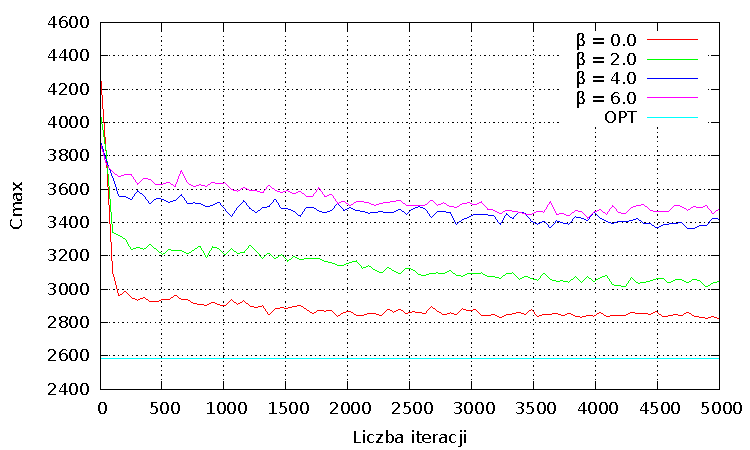
\includegraphics{./figures/inst01_rnd_beta_smooth.pdf}
    \caption{$ \beta = \{ 0, 2, 4, 6 \} $}
\end{figure}
\vspace{15mm}
Badany parametr $\beta$, wpływa na wagę atrakcyjności operacji ($\eta$), podczas wyboru następnego wierzchołka.
W przeprowadzonym teście algorytm zwraca najlepsze osiągi dla wartości $\beta = 0$.
Wraz ze wzrostem wartości tego parametru wyniki pogarszają się.
Oznacza to, że nie branie pod uwagę atrakcyjności poprawia efektywność algorytmu.
Jest to spowodowane tym, że algorytm ACO został zaprojektowany dla problemu TSP w którym uzyskanie rozwiązania nie wymusza odwiedzenia wszystkich krawędzi grafu, zatem wybieranie tych o małym koszcie sprzyja lepszym rozwiązaniom.
W problemie FSP wyklucza się możliwość pominięcia jakiejkolwiek operacji, dlatego wybieranie najpierw krótszych, nie sprzyja lepszym rozwiązaniom, a jedynie utrudnia dobre uszeregowanie zadań.

\newpage
\subsubsection{Różne wartości parametru $\alpha$.}
\vspace{6 mm}
\begin{center}
\begin{tabular}{|r|l|}
  \hline
  klasa instancji & losowa \\
  liczba zadań & 50 \\
  czasy operacji & $ \langle 5;100 \rangle $  \\
  liczba mrówek & 10 \\
  liczba pokoleń & 5000 \\
  $ \rho $ & 0.01 \\
  $ \beta $ & 2 \\
  $ q_0 $ & 0.8 \\
  $ \tau_0 $ & 0.001 \\
  \hline
\end{tabular}
\end{center}

\begin{figure}[h]
    \centering
    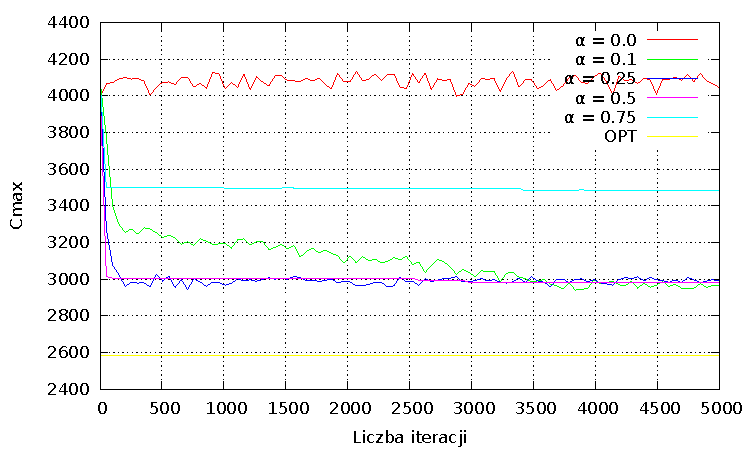
\includegraphics{./figures/inst01_rnd_alpha_smooth.pdf}
    \caption{$ \alpha = \{ 0.0, 0.1, 0.25, 0.5, 0.75 \} $}
\end{figure}
\vspace{15mm}
Parametr $\alpha$ wpływa na zanik feromonów na wszystkich ścieżkach oraz przyrost na najlepszej ścieżce w globalnej aktualizacji (wzór 5). Dla wartości $\alpha = 0$ algorytm zachowuje się jak losowy, ponieważ nie są przyznawane "nagrody" za najlepszą ścieżkę.
Wzrost wartości parametru zwiększa szybkość stabilizacji (nie optymalizacji).
Parametr wielkośći $\alpha = 0.5$ daje w pierwszych kilkudziesięciu iteracjach wartość stablilną przy dobrym wyniku.
Jednak zbytnie zwiększenie tego parametru ogranicza dalsze przeszukiwanie ścieżek, gdyż za bardzo zwiększa feromony na wcześnie odkrytych, dobrych ścieżkach.
Przy parametrze $\alpha = {0.1, 0,25}$ algorytm zwraca wartość zbliżoną do wartości przy $\alpha = 0.5$, jednak czas jej osiągnięcia jest dłuższy i algorytm nie osiąga pełnej stabilności.


\newpage
\subsubsection{Różne wartości parametru $q_0$.}
\vspace{6 mm}
\begin{center}
\begin{tabular}{|r|l|}
  \hline
  klasa instancji & losowa \\
  liczba zadań & 50 \\
  czasy operacji & $ \langle 5;100 \rangle $  \\
  liczba mrówek & 10 \\
  liczba pokoleń & 5000 \\
  $ \rho $ & 0.01 \\
  $ \beta $ & 2 \\
  $ \alpha $ & 0.1 \\
  $ \tau_0 $ & 0.001 \\
  \hline
\end{tabular}
\end{center}

\begin{figure}[h]
    \centering
    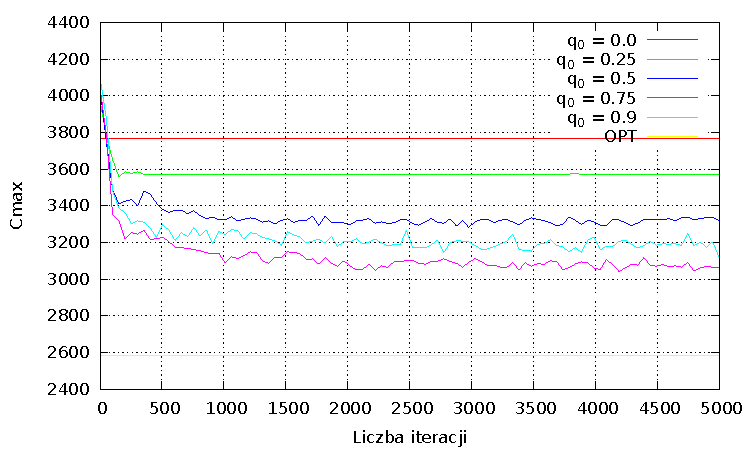
\includegraphics{./figures/inst_01_rnd_q0_smooth.pdf}
    \caption{$ q_0 = \{ 0.0, 0.25, 0.5, 0.75 \} $}
\end{figure}
\vspace{15mm}
Parametr $ q_0 $ wpływa na ruletkę - większa wartość oznacza częstsze korzystanie z ruletki.
Przykładowa wartość $ q_0 = 0.8 $ oznacza użycie ruletki w średnio 80\% przypadków zgodnie ze wzorem 2.
Przy zerowej wartości parametru nie ma poprawy jakości rozwiazań algorytmu, gdyż zawsze wybiera tę samą ścieżkę.
Poprawa jakości rozwiązań rośnie wraz ze wzrostem wartości $ q_0 $, jednak zbyt duży wpływ ruletki powoduje spadek jakości rozwiązań.
Potwierdzają to przeprowadzone testy, które wykazują lepsze wyniki dla parametru $ q_0 = 0.75 $ niż wartości $ q_0 = 0.9 $.

\newpage
\subsubsection{Różne wartości parametru $\tau_0$.}
\vspace{6 mm}
\begin{center}
\begin{tabular}{|r|l|}
  \hline
  klasa instancji & losowa \\
  liczba zadań & 50 \\
  czasy operacji & $ \langle 5;100 \rangle $  \\
  liczba mrówek & 10 \\
  liczba pokoleń & 5000 \\
  $ \rho $ & 0.01 \\
  $ \beta $ & 2 \\
  $ \alpha $ & 0.1 \\
  $ q_0 $ & 0.8 \\
  \hline
\end{tabular}
\end{center}

\begin{figure}[h]
    \centering
    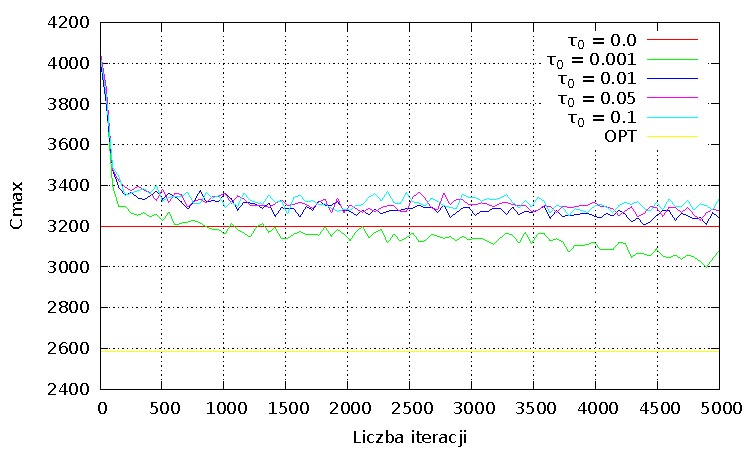
\includegraphics{./figures/inst_01_rnd_phinit_smooth.pdf}
    \caption{$ \tau_0 = \{ 0.0, 0.001, 0.01, 0.05, 0.1 \} $}
\end{figure}
Kolejna wartość sterująca programem - parametr $\tau_0$ - oznacza początkową wartość feromonu pomiędzy każdą parą wierzchołków grafu. Gdy $\tau_0 = 0$ wówczas, zgodnie ze wzorem 4,5 i 6 feromon aktualizowany jest jedynie na najlepszej ścieżce.


\newpage
\subsubsection{Różne wartości parametru $\rho$.}
\vspace{6 mm}
\begin{center}
\begin{tabular}{|r|l|}
  \hline
  klasa instancji & losowa \\
  liczba zadań & 50 \\
  czasy operacji & $ \langle 5;100 \rangle $  \\
  liczba mrówek & 10 \\
  liczba pokoleń & 5000 \\
  $ \tau_0 $ & 0.001 \\
  $ \beta $ & 2 \\
  $ \alpha $ & 0.1 \\
  $ q_0 $ & 0.8 \\
  \hline
\end{tabular}
\end{center}

\begin{figure}[h]
    \centering
    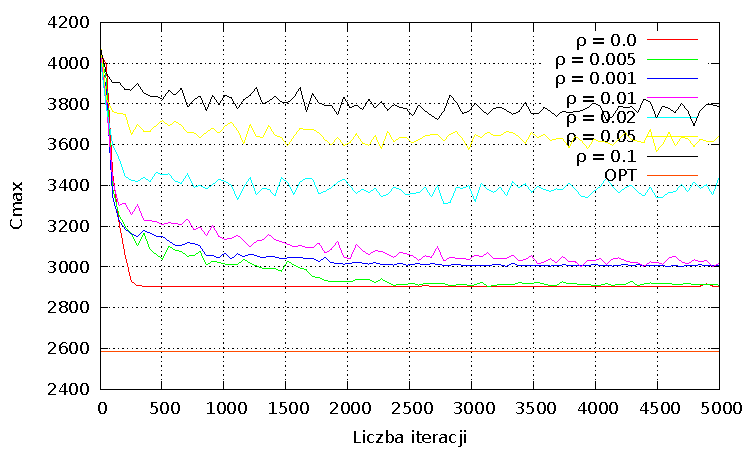
\includegraphics{./figures/inst_01_rnd_evapor_smooth.pdf}
    \caption{$ \rho = \{ 0.0, 0.01, 0.02, 0.05, 0.1 \} $}
\end{figure}


\newpage
\subsubsection{Różne wartości parametru liczby mrówek.}
\vspace{6 mm}
\begin{center}
\begin{tabular}{|r|l|}
  \hline
  klasa instancji & losowa \\
  liczba zadań & 50 \\
  czasy operacji & $ \langle 5;100 \rangle $  \\
  liczba pokoleń & 5000 \\
  $ \rho $ & 0.01 \\
  $ \tau_0 $ & 0.001 \\
  $ \beta $ & 2 \\
  $ \alpha $ & 0.1 \\
  $ q_0 $ & 0.8 \\
  \hline
\end{tabular}
\end{center}

\begin{figure}[h]
    \centering
    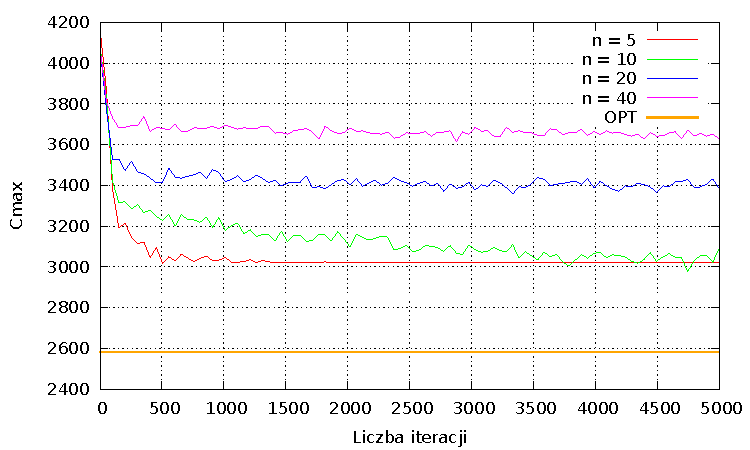
\includegraphics{./figures/inst_01_rnd_antno_smooth.pdf}
    \caption{liczba mrówek $= \{ 5, 10, 20, 40 \} $}
\end{figure}

\newpage
\section{Ocena efektywności}
Jakie parametry optymalne...

\section{Wnioski}
No sprawko jest piękne! :)


\end{document}
